\documentclass[mathserif]{beamer}

\usepackage{thesis}
\usepackage{pdfpages}

\title[Sampling from Probabilistic Submodular Models]
{Sampling from Probabilistic Submodular Models}

\author[Alkis Gotovos]{}


\newcommand{\btheta}{\*\theta}
\newcommand{\bu}{\*u}
\newcommand{\bw}{\*w}
\newcommand{\bv}{\*v}

\newcommand{\tab}[2]{%
\makebox[#1\linewidth][l]{#2}%
}

\begin{document}

\setbeamertemplate{background canvas}{}
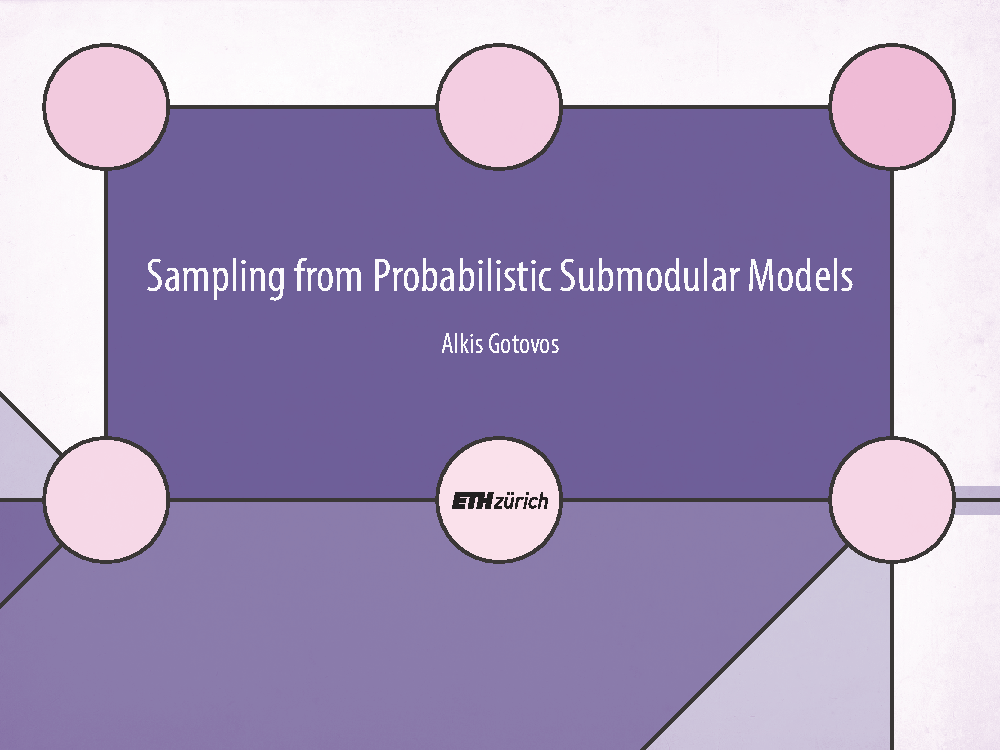
\includepdf[pages={1}]{title/title.pdf}
\setbeamertemplate{background canvas}{\includegraphics[width=\paperwidth]{figures/bg_no_line.png}}


\begin{frame}{The Cancer Genome Atlas}
\vspace{0.5em}
\centering
\includegraphics[width=2.5in]{figures/tcga.png}\\[-0.3em]
\hspace{12em}\qsource{cancergenome.nih.gov}
\end{frame}

\begin{frame}{The Cancer Genome Atlas}
\vspace{0.3em}
\centering
\includegraphics[width=3.85in]{figures/pathways_new.png}\\[-0.7em]
\hspace{22em}\qsource{Schultz et al., 2018}
\end{frame}

\begin{frame}{Modeling Interactions between Gene Mutations}
\centering
\includegraphics[width=3.7in]{figures/example1.pdf}
\end{frame}

\begin{frame}{Modeling Interactions between Gene Mutations}
\centering
\includegraphics[width=3.7in]{figures/example1_rep.pdf}
\end{frame}

\begin{frame}{Modeling Interactions between Gene Mutations}
\centering
\includegraphics[width=3.7in]{figures/example1_rep_group.pdf}

\vspace{3em}

\begin{itemize}
\item \tab{0.4}{Discrete optimization \hspace{0.3em} \includegraphics[width=0.13in]{figures/cross_mark.png}} \tab{0.15}{$\longrightarrow$} probabilistic models \hspace{0.3em} \includegraphics[width=0.13in]{figures/check_mark.png}
\vspace{0.7em}
\item \tab{0.4}{Classic pairwise models \hspace{0.3em} \includegraphics[width=0.13in]{figures/cross_mark.png}} \tab{0.15}{$\longrightarrow$} higher-order interactions \hspace{0.3em} \includegraphics[width=0.13in]{figures/check_mark.png}
\vspace{0.7em}
\item \tab{0.4}{Deep nets \hspace{0.3em} \includegraphics[width=0.13in]{figures/cross_mark.png}} \tab{0.15}{$\longrightarrow$} structured prior assumptions \hspace{0.3em} \includegraphics[width=0.13in]{figures/check_mark.png}
\end{itemize}
\end{frame}

\begin{frame}{Probabilistic Submodular Models}

\begin{center}
Distributions over $S \subseteq V = \{1,\ldots,n\}$

\vspace{0.8em}
\qboxa{
$p(S; \btheta) = \displaystyle\frac{1}{Z(\btheta)}\exp \big( F(S; \btheta) \big)$
}
\end{center}
\vspace{2em}

\begin{columns}
\begin{column}{0.54\textwidth}
\begin{itemize}
\item $F : 2^V \to \mathbb{R}\ $ is sub- or supermodular
\item $Z\ $ is the normalizer
\item $\btheta\ $ is a parameter vector
\end{itemize}
\end{column}
\begin{column}{0.39\textwidth}
\begin{itemize}
\item Ising model (log-supermodular)
\item DPP (log-submodular)
\end{itemize}
\end{column}
\end{columns}

\end{frame}

\begin{frame}{Learning \& Inference}

\end{frame}

\begin{frame}{Thesis Topic}
$\rightarrow\ \ $ Investigate the use of sampling to perform approximate inference in PSMs

\vspace{4em}

\centering
\uncover<2->{%
\only<1-2>{\includegraphics[width=\textwidth]{figures/chapters.pdf}}
\only<3>{\includegraphics[width=\textwidth]{figures/chapters1.pdf}}
}
\end{frame}

\begin{frame}{Improved Mixing using Semigradients}
\centering
\includegraphics[width=\textwidth]{figures/chapters2.pdf}
\end{frame}

\begin{frame}{Modeling Interactions between Cancer Mutations}
\centering
\includegraphics[width=\textwidth]{figures/chapters3.pdf}
\end{frame}

\end{document}
